%!TEX TS-program = xelatex 
%!TEX TS-options = -output-driver="xdvipdfmx -q -E"
%!TEX encoding = UTF-8 Unicode
%
%  seminar_1
%
%  Created by Mark Eli Kalderon on 2010-01-17.
%

\documentclass[11pt]{article} 

% Definitions
\newcommand\myauthor{Mark Eli Kalderon} 
\newcommand\mytitle{Empiricism and the Philosophy of Mind}
\newcommand\mysubtitle{Parts I and II}

% Packages
\usepackage{url}
\usepackage{txfonts}
\usepackage{color}
\definecolor{myblue}{rgb}{0.8,0.8,1}

% Define discussion environment
\makeatletter\newenvironment{discussion}{%
   \noindent\begin{lrbox}{\@tempboxa}\begin{minipage}{\columnwidth}\setlength{\parindent}{1em}}{\end{minipage}\end{lrbox}%
   \colorbox{myblue}{\usebox{\@tempboxa}}
}\makeatother

% XeTeX
\usepackage[cm-default]{fontspec}
\usepackage{xltxtra,xunicode}
\defaultfontfeatures{Scale=MatchLowercase,Mapping=tex-text}
\setmainfont{Hoefler Text}
\setsansfont{Gill Sans}
\setmonofont{Inconsolata}

% Title Information
\title{\mytitle\\
\mysubtitle}
\author{\myauthor} 
\date{} % Leave blank for no date, comment out for most recent date

% PDF Stuff
\usepackage[plainpages=false, pdfpagelabels, bookmarksnumbered, backref, pdftitle={\mytitle}, pagebackref, pdfauthor={\myauthor}, xetex, colorlinks=true, citecolor=gray, linkcolor=gray, urlcolor=gray]{hyperref}

%%% BEGIN DOCUMENT
\begin{document}

% Title Page
\maketitle

% Layout Settings
\setlength{\parindent}{1em}

% Main Content

\begin{figure}[htbp]
	\centering
		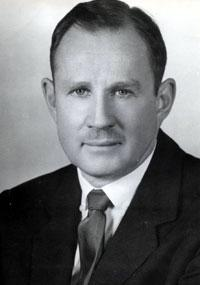
\includegraphics[scale=0.5]{../graphics/sellars.jpeg}
	\caption{Wilfrid Sellars}
	\label{fig:sellars}
\end{figure}

\section{An Ambiguity in Sense-Datum Theories} % (fold)
\label{sec:an_ambiguity_in_sense_datum_theories}

\emph{Section 1}: Sellars aims to attack ``the whole idea of givenness,'' but proposes to do so by beginning with a special case---the given as it arises in sense-datum theories. Sellars doesn't explicitly tell us what the given is. No doubt he assumed that his audience at the University of London Special Lectures in Philosophy in March of 1956 knew, at least approximately, what he meant by the given. Whatever the merits of that assumption, it is less likely to be the case for us now. Instead, we must rely on the scattered clues provided by the text.

In attacking the given, Sellars doesn't mean to undermine the distinction between ``\emph{inferring} that something is the case and, for example, \emph{seeing} it to be the case''. Notice the distinction is between inferring and propositional seeing, seeing-\emph{that}. And since seeing is marked out as just an example, if a prominent one, the distinction is presumably between judgements formed on the basis of inference and non-inferential judgments paradigmatically (if not inevitably) formed on the basis of perception. ``The given'' is meant to carry ``substantial theoretical commitments'' that go beyond this commonplace.

\emph{Section 2}: Sellars sketches the framework of the classical sense-datum theory. He focuses on the act--object structure that sense-datum theorists attribute to sensings understood as conscious episodes. On the one hand, there is the act of awareness or \emph{sensing}, and on the other hand there is the object of that awareness, the \emph{sense content}. Thus Moore in sensing the blue bead, we can distinguish the act of awareness---Moore's sensing, and what Moore was aware of---the sense content of that awareness (which presumably includes the bead's shape and color).

In addition, Sellars makes the suggestion that different sense modalities (visual sensing, tactual sensing, etc.) may be distinguished by their sense contents (as opposed to positing distinct kinds of sensings.) This is controversial given that there are sense contents available to distinct sens0ry modalities (we can see a shape and feel it).

\emph{Section 3}: What's the ontological status of sense contents? Are they facts or particulars? This forms the basis of a dilemma:
\begin{enumerate}
	\item It is \emph{particulars} which are sensed. Sensing is not knowing. The existence of sense-data does not \emph{logically} imply the existence of knowledge.
	\item Sensing \emph{is} a form of knowing. It is \emph{facts} rather than \emph{particulars} which are sensed.
\end{enumerate}

Sellars remarks that on the first alternative sensing a sense content (where sense contents are particulars) is a \emph{non-epistemic} fact. This is important since, as we shall see, the myth of the given as it arises for the sense-datum theory is claimed to be analogous to Moore's naturalistic fallacy. Just as Moore claimed that it was a mistake to infer normative truths from (non-normative) natural truths, Sellars claims that it is a mistake to infer epistemic truths from non-epistemic truths. So what's an ``epistemic fact'' here? It is at least clear that facts about a subject's knowledge count as epistemic facts. So it is an epistemic fact about me that I know, say, that there was an earthquake in Haiti. Perhaps it is also the case that epistemic facts involve propositional states of a subject. But is the domain of epistemic fact broader than this? Suppose I justifiably believe that p, even if I fail to know that p. Would this count as an epistemic fact in Sellars sense? For the most part this won't matter since Sellars focus will be on the non-propositional character of sense data.

% section an_ambiguity_in_sense_datum_theories (end)

\section{Another Language?} % (fold)
\label{sec:another_language_}

% section another_language_ (end)

\end{document}